\documentclass[a4paper,12pt]{thesis}

\usepackage[utf8]{inputenc}

\usepackage{blindtext}


\usepackage[onehalfspacing]{setspace}

\usepackage{adjustbox}
\usepackage[ngerman]{babel}
\usepackage[T1]{fontenc}
\usepackage{amsfonts}
\usepackage{amsmath}
\usepackage{mathtools} 
\usepackage{mathabx}
\usepackage{graphicx}
\usepackage[table]{xcolor}
\usepackage{longtable}
%\usepackage{hyperref}

\usepackage{setspace}

\usepackage{color}
\usepackage{transparent}

\usepackage{tikz}
\usetikzlibrary{positioning}
\usetikzlibrary{arrows,calc}
%\usepackage{pgfplots} % LaTeX
\usepackage{colortbl}
%\usepackage{pgfplotstable}
\usepackage{booktabs, colortbl}

\usepackage{eurosym}

\usepackage{csvsimple}

\usepackage[authoryear]{natbib}
%\bibliographystyle{apalike}
\usepackage[hidelinks]{hyperref}
\bibliographystyle{apalike}

\newcommand*{\captionsource}[2]{%
	\caption[{#1}]{%
		#1%
		\\\hspace{\linewidth}%
		\textbf{Quelle:} #2%
	}%
}

\tikzset{
%Define standard arrow tip
>=stealth',
%Define style for different line styles
help lines/.style={dashed, thick},
axis/.style={<->},
important line/.style={thick},
connection/.style={thick, dotted},
}


\begin{document}

%%% TITELSEITE %%%

\begin{center}								% Beginn einer center-Umgebung. Der Text innerhalb der center-Umgebung wird zentriert. Ansonsten wird Blocksatz verwendet
	\begin{LARGE}								% LARGE beschreibt eine Schriftgröße in Latex. Der Standard ist \normalsize. Eine übersicht der Schriftgrößen steht z.B. auf der Seite: https://www.latex-kurs.de/fragen/schriftgroesse.html 
		Räumliche Vorhersage des urbanen Radverkehrs mit Machine Learning					% Text, der nun zentriert und in größerer Schrift geschrieben wird 
	\end{LARGE}								% Die Verwendung der Schriftgröße LARGE wird beendet. Es gilt ab jetzt wieder die normale Schriftgröße.
	
	\vspace{\fill}								% Befehl, der den vertikalen Platz (vspace) "füllt" 
	
	\begin{large}								% Der folgende Text hat nun die Schriftgröße large 
		Maximilian Samuel Weinhold\\					% Durch ein \\ wird eine neue Zeile angefangen. 
		Economics, 7. Semester\\
		505314\\
		mweinhol@uni-muenster.de\\
		
		\vspace{\fill}
		
		Masterarbeit zur\\
		räumlichen Vorhersage von Fahrrad-Verkehrsdaten\\
		Wintersemester 2022\\
		Institut für Verkehrswissenschaft\\
		Prof. Dr. Gernot Sieg\\
	\end{large}
	
	\thispagestyle{empty}						% Definiert den Stil für diese Seite. empty bedeutet, dass keine Seitenzahl auf der Seite gedruckt wird. 
	
\end{center}								% Ab nun wird wieder Blocksatz verwendet

\newpage									% Seitenumbruch. Es beginnt eine neue Seite


%\chapter*{Tabellen und Abbildungen}\addchapmark{Tabellen und Abbildungen}
\onehalfspacing	
\thispagestyle{empty}	
\tableofcontents

\begingroup
\let\clearpage\relax
\listoffigures
\listoftables
\endgroup

\chapter{Einleitung}

Vielerorts erlebt der Individualverkehr eine Renaissance des Fahrrads, eingeleitet durch ein umweltbewusstes Umdenken. So ist laut \cite{Eisenberger2015} und dem Verband der Zweirad Industrie \cite{ZIV2022} der Bestand an Fahrrädern in Deutschland von 72 Mio. in 2015 auf 81 Mio. in 2021 angestiegen. Der anhaltende Boom hat viele Gründe. Im Vergleich zum Auto ist die bewegungsintensivere Fortbewegung auf dem Fahrrad gesünder, schont die Umwelt und das Portmonee. Zuletzt wurde dieser Boom weiter befeuert durch die Corona Pandemie.\\
Doch mit einem Anstieg an Fahrrädern steigt auch der Bedarf nach ausgebauten Fahrradwegen. So unterstützt das Bundesministerium für Verkehr und digitale Infrastruktur \cite{VerkehrunddigitaleInfrastruktur2020} die Länder und Gemeinden durch eine direkte Hilfe in Höhe von 660 Mio. Euro bis 2023 beim Ausbau von Radwegen. Gleichzeitig besteht die Möglichkeit eines steigenden Risikos für Unfälle, wenn mehr Fahrradfahrer im Stadtverkehr unterwegs sind.\\
Dies sowie der genaue lokale Bedarf und die Auslastung von Fahrradwegen muss bei der Planung der Infrastruktur beachtet werden. Deswegen ist die Forschungsfrage dieses Projekt Studiums, wie man das Fahrradverkehrsvolumen und den damit verbundenen Bedarf von Radwegen messen kann. Ist es möglich ein räumliches Modell zu entwickeln, dass für ein vollständiges Straßennetz oder für ausgewählte flexible Knotenpunkte zu bestimmten Zeiten Vorhersagen zum Fahrradverkehr machen kann und lassen diese auch zusätzlich die gefährlichsten Stellen für Fahrradunfälle erkennen?\\
Dazu beginnt diese Hausarbeit mit einem ausführlichen Einblick in die bestehende Literatur, kategorisiert nach Datengrundlagen und Methoden. Häufig verwendete Methoden werden im Nachgang näher beschrieben. Die Diskussion versucht mit dem erworbenen Wissen, einen Weg zu finden, mit dem sich ein Modell entwickeln ließe, das die gestellten Fragen potentiell beantworten könnte und gibt damit Ausblick auf eine kommende Master Arbeit.

\chapter{Literaturüberblick}

Die Auslastung von Fahrradwegen bzw. das Aufkommen von Fahrrädern beruht im Wesentlichen auf der individuellen Entscheidung eines jeden Fahrers, das Fahrrad einer anderen Transport Alternative vorzuziehen. Versteht man die Faktoren, aus denen sich diese Entscheidung zusammensetzt, dann kann man leichter eine solche Entscheidung vorhersagen. Mit einer Zusammenfassung der bisherigen Literatur wollen \cite{Heinen2010} diese Faktoren finden, wobei sie sich auf Pendler beschränken. Zum einem ist einer dieser Faktoren die bauliche Substanz, die nicht nur die Radwege sondern auch Abstellmöglichkeiten und Ampeln wie auch Verkehrsschilder beinhaltet. Zum anderem spielt das Wetter eine große Rolle. Einen negativen Effekt hat die Rate der Autobesitzer und natürlich auch die Verfügbarkeit anderer Transportmöglichkeiten.\\

\section{Gegenstand der Forschung}

Seitdem erschienen zahlreiche weitere empirische Studien, die unser Bild konkretisieren. Diese Studien lassen sich nach Datenquellen und Methoden kategorisieren. Die meisten nutzen vier verschiedene Datengrundlagen zum Fahrradverkehr in Verbindung zu Daten mit anderen Faktoren wie dem Wetter. Die vier Datenquellen zum Fahrradverkehr stammen von Fahrradzählstation, einer Induktionsschleife die darüber fahrende Räder verifiziert, Daten von Bike Sharing Diensten, Daten verschiedener GPS und Handy Applikationen und auch Unfallstatistiken von Fahrrädern finden Beachtung in der empirischen Analyse.\\

\subsection{Forschung mit Zählstationen}

In Deutschland findet sich eine weite Verbreitung von Fahrradzählstationen verschiedener Städte, deren Daten oft öffentlich einsehbar sind. Deswegen wäre eine Verwendung dieser Datengrundlage überaus praktisch. Studien, die ähnliche Daten verwenden, sind zB \cite{Holmgren2017}, \cite{Broucke2019}, \cite{Wessel2020} und \cite{Goldmann2021}. Auf die Arbeit von \cite{Wessel2020} geht diese Hausarbeit später ein, denn dort liegt ein starker Fokus auf Wetter Daten. \cite{Holmgren2017} verwenden tägliche Daten von 2006 bis 2014 aus Malmö, ebenfalls wie später bei \cite{Wessel2020} verbunden mit Wetterdaten, Feiertagen und Schulferien. Als Methode zur Auswertung dieser Daten und zur Schätzung des Fahrradaufkommens verwendeten sie Zufallsbaum Regressionssysteme, Support Vector Regression, eine lineare Regression und ein Multiy Layer Perceptron also ein neuronales Netz. Im Vergleich dieser Methoden erzielen sie die treffsichersten Resultate mit einem Regressionsbaum und der Support Vector Regression, die auf quadratische und kubische Kernels zurückgreift. Mithilfe des Support Vector Regressionssystems kommen sie auf ein Bestimmtheitsmaß R$^2$ von 86,9 \%.\\
Um diese Methoden zu vergleichen nutzen \cite{Holmgren2017} die Cross Validation. Ähnlich gehen \cite{Broucke2019} vor, unter Verwendung von Daten von 12 Zählstationen aus Brüssel. Sie verbinden diese Daten mit temporalen, geographischen und metereologischen Daten. Ebenfalls verwenden sie eine Support Vector Regression, die auf einer radialen Basis Funktion aufbaut, um eines ihrer vier Modelle zu berechnen. Für die anderen drei verwenden sie Random Forests Regression, welche auf Zufallsbäume aufbaut, ein gradient Boosting Modell und ein voll verknüpftes neuronales Netzwerk. Letzteres beinhaltet 2 Schichten mit einmal 28 und einmal 14 Knoten, die die ReLU (Rectified Linear Unit) Funktion als Aktivierung verwenden. Von allen Modellen mit Wetterdaten erzielt das neuronale Netzwerk hier den niedrigsten RMSE (Root Mena Squared Error) und schneidet somit am besten ab.

\subsection{Forschung mit Bike Sharing Diensten}

Die überragende Mehrheit an Studien zur Schätzung und Vorhersage des Fahrradverkehrs verwendet Daten von Bike Sharing Diensten, dazu zählen \cite{Kaltenbrunner2010}, \cite{Xu2013}, \cite{Li2015}, \cite{Mitchell2018PredictingBT}, \cite{Colace2020}, \cite{Gao2022} und \cite{Li2022}. Dies ist natürlich immer noch nur eine Auswahl an Studien. Die Literatur zu Bike Sharing Systemen ist sehr ausführlich. Eine weitere Übersicht hierzu findet sich bei \cite{Mitchell2018PredictingBT}.\\
\cite{Kaltenbrunner2010} nutzen z.B. Daten von 400 öffentlichen Rad Ausleihstationen in Barcelona. Ihre Studie hegt die Absicht, die Effizienz des bestehende Verleih Systems in Barcelona, das zu dem Zeitpunkt um die 180000 Abonnenten hatte, zu verbessern. Hier geht es also eher darum, vorherzusagen, wie viele Fahrräder sich in welcher Ausleihstation zu welchem Zeitpunkt befinden, um den Nutzern detaillierte Informationen zu geben.\\
Eine ähnliche Motivation haben \cite{Xu2013}. Diese verwenden Daten ihren Aussagen zufolge des größten öffentlichen Bike Sharing Systems der Welt in Hangzhou in China. Ihr Datensatz beinhaltet die aufgezeichnete Auslastung der Stationen einiger Tage und Wochen zuvor, sowie Daten zum aktuellen und vergangenem Wetter und Informationen über Feiertage. Diesen Datensatz normalisieren und clustern sie mit der k-means Cluster Methode. Darauf wenden sie Support Vector Machines an, um die Gewichte der beschriebenen Estimatoren zu finden. Dieses hybride Modell hat nur noch eine Fehlerrate von 3,57 \% vergleicht man dessen Vorhersagen, mit den tatsächlich eingetretenen Auslastungen.\\
\cite{Li2015} stellen hier ein Paper zur Verfügung das ähnlich funktioniert. Auch sie wollen eine Ausbalancierung der Fahrradbestände an allen Stationen in New York und Washington DC erleichtern. Und genau wie \cite{Xu2013} unterteilen sie die Stationen in Cluster. Für diese Cluster wollen sie Vorhersagen machen, was zu robusteren Ergebnissen führt, als wenn man für jede einzelne Station Vorhersagen bildet. Zusätzlich verwenden \cite{Li2015} Wetter Beobachtungen in ihrem Datensatz. Darauf wird ein Gradient Boosting Regression Tree angewendet. Gradient Boosting kurzläufige zufällige Entscheidungsbäume, die der Reihe nach auf den Fehlerterm des vorherigen Beruhen und diesen versuchen zu verbessern.\\
Auf Cluster Level Bike Sharing geht auch \cite{Mitchell2018PredictingBT} ein. Er evaluiert verschiedene Machine Learning Methoden miteinander: Random Forests, Fast Feed Forward Neural Networks, Deep Residual Networks und Recurrent Neural Networks.  Dabei schlagen sich die Feed Forward Neural Networks am besten.\\
Einen besonderen Ansatz verfolgen \cite{Colace2020}, die Aufnahmen von Überwachungskameras in ihrer Analyse mit aufnehmen.\\
Eine besonders aktuelle Analyse stammte von \cite{Gao2022}. \cite{Gao2022} sind hierbei die Ersten von den bisher genannten, die mehr Informationen als nur Wetterberichte in seiner Analyse aufnehmen. Aufbauend auf Daten zu 2098 Fahrradstationen aus Seoul nehmen sie in ihr Modell z.B. Feinstaubbelastungen mit auf, was \cite{Hong2022} und \cite{ZHAO2018826} als relevanten Faktor gezeigt haben. Daneben inkludieren sie auch Verkehrsdaten, Corona Fälle und Sozioökonomische Daten, Verkehrsunfälle und Saisonalität. Darauf wenden sie lineare Regressionen, k-nearest neighbour (knn), Random Forests und Support Vector Machines an. All diese Methoden wurden in R angewendet. Diese Modelle vergleichen sie mit einem Validation-Set-Schnitt von 75 \% für das Trainings Set und 25 \% für das Test Set. Damit betreiben \cite{Gao2022} eine Feature Selection, die auf den Boruta Algorithmus zurückgreift. Das Ziel von Feature Selektion ist, am Ende ein Modell zu haben, dass nur auf statistisch relevante Variablen zurückgreift. Dazu erstellt der Boruta Algorithmus nach \cite{Kursa2010} verschiedene unabhängige Bagging Samples, zieht daraus Klassifikationsbäume und beurteilt die Features nach Verlust an Akkurarität. Die relevantesten Variablen waren das Wetter und die Anzahl der Corona Fälle. Mit einer 10-fold Cross Validation fand man heraus, dass sich die Support Vector Machines und die Random Forests am besten geschlagen haben. So lässt sich mit Random Forests ein Test R$^2$-Wert von 93 \% erreichen und mit SVM ein Test R$^2$-Wert von 90 \%, was beides sehr gute Werte sind. Dabei spielten auch die sozioökonimische Daten eine Rolle, die im Gesamten zwar wenig Relevanz hatten, aber Unterschiede zwischen den Docking Stationen erklären konnten.\\ 
\cite{Li2022} möchten nicht nur den Bestand von Rädern an fixen Fahrrad Ausleihstationen vorhersagen, sondern die generelle Nutzung und das Verkehrs Volumen von Leihrädern in einem Gebiet berechnen. Dazu verwenden sie Daten von festen Fahrradstationen in Chicago und New York und Daten von Ausleihsystemen mit frei stehenden Fahrrädern die GPS Daten speichern in Singapore und New Taipei City. Jede Stadt zerteilen sie in ein Raster und wenden darauf convolutional neural Networks an, die auch oft für die Bilderkennung verwendet werden. Das Ergebnis dessen ist in der Abbildung \ref{LiBild} zu sehen.\\
\begin{figure}[!ht]
	\centering
	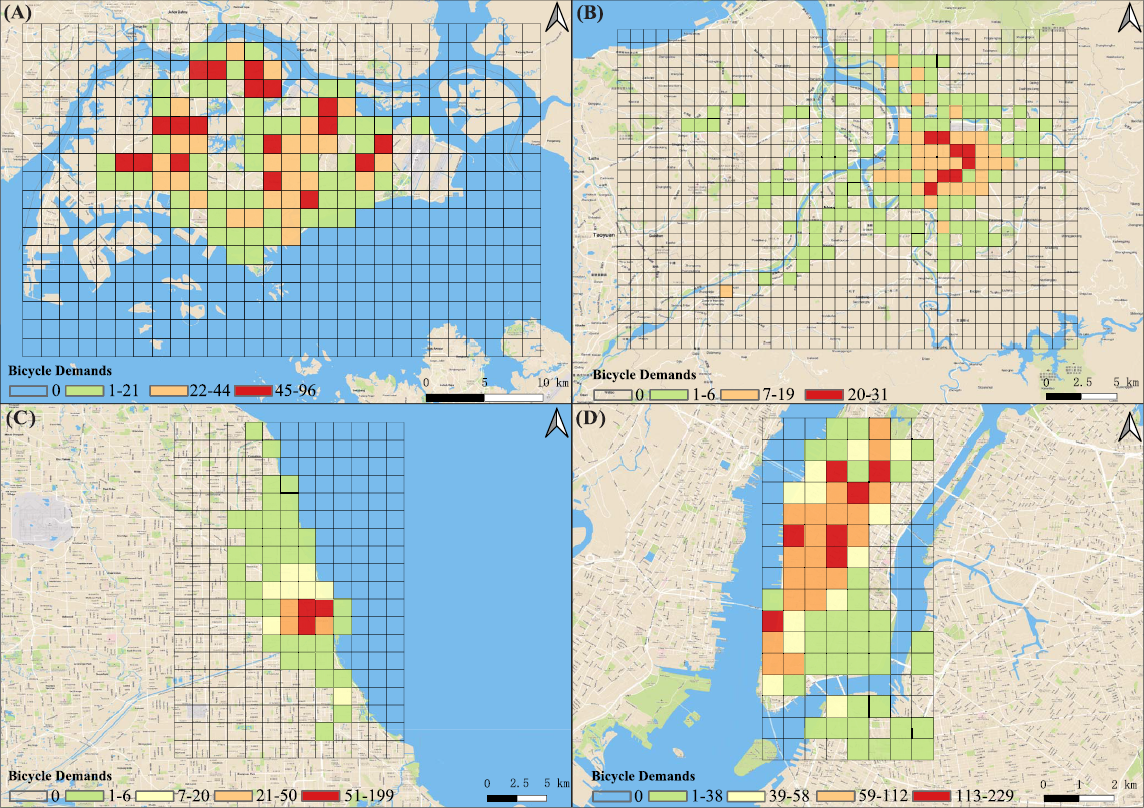
\includegraphics[width=\textwidth]{Plots/Li2022.png}
	\captionsource{Anzahl der Leihräder (A) Singapore zwischen 8-9 Uhr am 25. Juni 2017; (B) New Taipei City zwischen 18-19 Uhr am 1. August 2018; (C) Chicago zwischen 16-18 Uhr am 26. August 2019; (D) New York zwischen 17-18 Uhr am 9. Juni 2014.}{
		\cite{Li2022}
	}
	\label{LiBild}
\end{figure}
Eine Besonderheit dieser Arbeiten, die alle auf Daten von Bike Sharing Diensten beruhen, ist, dass sie mehr Datenpunkte in einer Staat zur Verfügung haben, da ein Netz von Leihstation eine höhere Dichte haben muss. So können \cite{Gao2022} z.B. 2098 Stationen in einer Stadt beobachten, während \cite{Broucke2019} z.B. nur 12 Zählstationen in einer Stadt zur Verfügung haben. Deshalb ergibt das Clustering von Bike Sharing Daten Sinn, wie es zB \cite{Xu2013} und \cite{Li2015} vornehmen.\\
Modelle die auf Zählstationen beruhen, können das gesamte Verkehrs Volumen an bestimmten Punkten messen und schätzen. Die hier kennen gelernten Modelle, die auf Bike Sharing Daten zurükckgreifen, können das nicht, sondern ermitteln nur das Verkehrs Volumen, das von diesen Mieträdern kommt, dafür aber immer für das vollständige Mietradsystem. Interessant wäre die Frage, wie Mietradverkehr und Verkehr von Rädern in Privatbesitz miteinander korrelieren. Wer mit dem Fahrrad regulär pendelt, für den ist der Besitz eines Fahrrads langfristig kostengünstiger. So kann es sein, dass Spitzen in beiden Varianten von einander abweichen, weil Mieträder möglicherweise eher touristischen statt utilitaristischen Zwecken dienen. Mietraddaten allein sind also kein ausreichendes Mittel, um den gesamten Fahrrad Verkehr zu modellieren. Möglicherweise gäben aber Handy Daten mehr Aufschluss.

\subsection{Forschung mit GPS und Handy Daten}


Schon im vorangegangenen Abschnitt zu den Daten von Bike Sharing Systemen hat \cite{Li2022} GPS Daten von Leihfahrrädern für seine Analyse genutzt. Doch das ist nicht die einzige Möglichkeit um an GPS Daten zu kommen. Ein weiterer Weg sind Handy Applikationen, die beständig GPS Koordinaten aufzeichnen und damit Bewegungsprofile erstellen. \cite{Romanillos2016} stellen solche Studien vor, die auf GPS Daten von Fitness und Leisure Applikationen zurückgreifen.\\ 
Eine der ersten Arbeiten wurde von \cite{Harvey2007} mit der Absicht erstellt, durch ihr Modell eine Priorisierung von Fahrradinfrastruktur zu ermöglichen. Dazu verwendeten sie noch GPS Logging Ausrüstung bei 51 Teilnehmern in einem Zeitraum von 3 Wochen in South Minneapolis, um favorisierte Radstrecken aufzuzeichnen. Neben der niedrigen Stichprobenmenge war diese Studie noch mit dem Problem des GPS Cleanings konfrontiert, das zu Positionsabweichungen führen kann. Diese Probleme wurden von Folgestudien wie von \cite{Menghini2010} erstmals behoben, die in Zürich Daten von 2400 Teilnehmern hatten und mit einem verbessertem Detection Algorithmus auch Probleme des GPS Post Processing behoben haben.\\ 
Das Prinzip der GPS Aufzeichnung entwickelte sich weiter und \cite{Reddy2010} verwendeten erstmals Handys als GPS Logging Geräte. Dazu verwenden sie Daten der App Biketastic. Das Problem bei Bike Logging Apps ist, dass hier eher Fahrrad Routen aufgezeichnet werden, die der Erholung dienen und nicht unbedingt dem alltäglichen utilitaristischen Stadtverkehr. Die Nutzung dieser Daten gibt also nicht Aufschluss über den gesamten Fahrradverkehr. Bei der hier genutzten Applikation Biketastic ist das jedoch anders, denn Biketastic wird speziell von Pendlern genutzt, um nicht nur GPS Daten aufzuzeichnen, sondern auch Fotos und Audioaufnahmen der Handys, um Straßen mit signifikant hohen Lärm ausfindig zu machen und so lauten Straßenverkehr in das Modell aufzunehmen. Bei der Evaluation stellte man schnell fest, dass Nutzer der App dazu tendierten, diese nur für lange Strecken zu nutzen, und sich nicht die Mühe machen, die App auf dem Handy zu betätigen, wenn man eine Strecke von unter einer Meile zurück legen wollte.\\
Eine weitere Studie stammte von \cite{Broach2012}, aber auch hier ist die Anzahl der Studienteilnehmer mit knapp über 164 gering. Weitere Studien in dem Bereich stammen von \cite{Musakwa2016}, \cite{Pritchard2018}, \cite{Lee2020} und \cite{Alattar2021}. Eine der aktuelleren Studien ist von \cite{Alattar2021}. Sie verwenden Daten, die durch die Fitness App Strava in Glasgow 2017 bis 2018 gewonnen wurden, um den Einfluss des Straßenlayouts auf die Routenwahl der Fahrer zu untersuchen. Dabei bauen sie auf ein räumliches Modell, das an bestimmten Straßenknotenpunkten stündliche durchgehende Fahrradfahrten nach Straße, Abfahrtsort und Zielort betrachtet. Um zu testen, wie gut die Strava Daten den Tatsächlichen Radverkehr abbilden, wurde mit insgesamt 36 temporären Zählstation das Radverkehrsvolumen über zwei Tage stichprobenartig verglichen. Neben den Daten von Strava nutzten die Autoren das Python Paket OSMnx, dass direkten Zugang zu Open Street Map bietet. Open Street Map bietet umfassende Information über Glasgows Straßennetz und so können die Knotenpunkte mit dem Straßennetz verglichen werden. Das daraus resultierende Ergebnis ist in Abbildung \ref{Alattar_2021} zu sehen.
\begin{figure}[!ht]
	\centering
	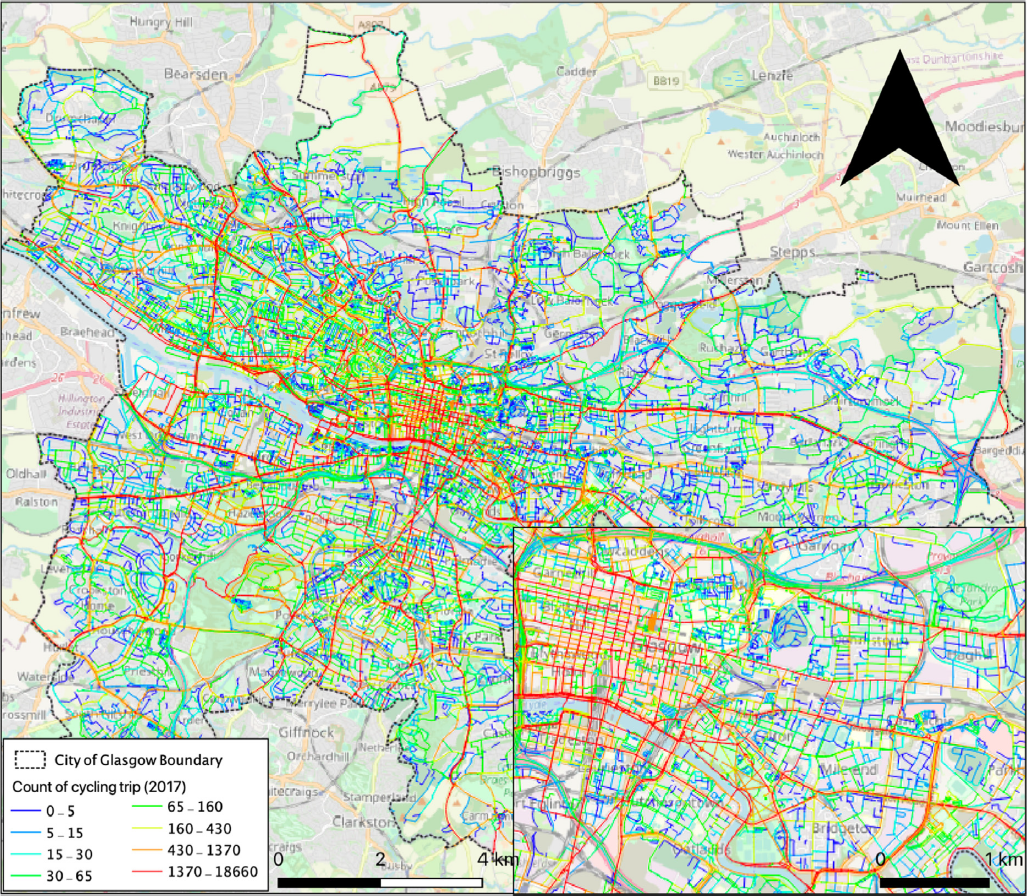
\includegraphics[width=\textwidth]{Plots/Alattar2021.png}
	\captionsource{Fahrradaufkommen für Glasgow 2017}{
		\cite{Alattar2021}
	}
	\label{Alattar_2021}
\end{figure}
Auf diese Daten kann nun eine Regression angewendet werden, deren erklärende Variablen logarithmerte Indikatoren der Zentralität innerhalb des Knotennetzwerkes sind, die die Anzahl der Fahrradtrips erklären sollen. Bei diesem Regressionsmodell kommt ein Erklärungswert R$^2$ von 42 \% zustande, was im Vergleich zu vorherigen Werten gering ist. Ein interessanter Forschungspunkt den \cite{Alattar2021} hätten hier noch verfolgen können, wäre wie sich die Vorhersagekraft ändert, wenn man Wetter, Feier und Ferientage in das Modell mit aufnimmt.\\
Im Überblick zeigen sich häufige Schwächen von Studien, die Handy Applikationsdaten nutzen, wie den Strava Datensatz. Zunächst unterliegen solche Apps häufig einer Selbstauswahl der Probanden. So sind z.B. in dem Datensatz von \cite{Alattar2021} Frauen unterrepräsentiert. Häufig dienen diese Apps der sportlichen Betätigung und nicht der Anfahrt zum Arbeitsplatz. Zudem sind ihre Daten schwer zugänglich.


\section{Aspekte der Forschung}

Die Prädikatoren eines Modells spielen eine große Rolle, denn mit der Auswahl der richtigen Prädikatoren steht und fällt die Validität des Modells. Deswegen klärt ein gesonderter Literaturüberblick die Tragweite einzelner Variablen, die möglicherweise das Aufkommen an urbanen Fahrradverkehr erklären können. Wichtiges Attribut eines Prädikators ist zudem die Datenverfügbarkeit. 

\subsection{Aspekt zum Wetter}

Wetter und Wetterelastizität


Vielmals begegnet in der bisherigen Literatur Betrachtung sind Wetter Daten, so z.B. bei \cite{Holmgren2017}, \cite{Broucke2019}, \cite{Li2015}. Literatur, die sich speziell mit diesem Zusammenhang beschäftigt findet sich bei \cite{Wessel2020}. Dabei hat er sich z.B. im Gegensatz zu \cite{Nankervis1999}, der sich auch mit dem Zusammenhang von Wetter und Fahrrad Aufkommen beschäftigt, gezielt mit dem Zusammenhang von Wettervorhersagen beschäftigt. Auch \cite{Meng2016} untersucht diesen Zusammenhang.\\
Jedoch während \cite{Meng2016} Daten einer Umfrage von 553 Fahrradfahrern in Singapore verwendet, stützt sich \cite{Wessel2020} auf umfangreichere Daten von 188 Fahrradzählstationen in 37 deutschen Städten, die stündlich zählen. Daten zum aktuellen Wetter stammen vom Deutschen Wetterdienst. Daten über Wettervorhersagen stammen aus der ARD Mediathek, der abendlichen Tagesschau um acht Uhr. Die Aufzeichnungen der Wettervorhersagen worden dabei manuell ausgewertet, wobei der deutsche Raum in sechs Hemisphäre Nordwest, Nordost, mittlerer Westen und mittlerer Osten so wie Südwest und Südost unterteilt wurde und die Städte in die korrespondierende Hemisphäre eingeteilt worden sind nach folgenden Wetter Klassifikationen: klarer Himmel, leichte Bewölkung, schwere Bewölkung, Regen, Schneefall, Gewitter und zusätzlich Wind, Rutschgefahr, Vereisungen, Überflutung und generelle Warnungen. Neben dieser manuellen Einschätzung der Bewölkung wurde zusätzlich eine digitale automatisierte Einschätzung verwendet, die sich auf die Dunkelheit der Pixel des Kartenmaterials bezieht.\\
Aufbauend auf diesen Daten nutzt \cite{Wessel2020} ein log-lineares Regressionsmodell und ein negativ binomiales Regressions Modell. Das letztere Modell geht auf \cite{Hausman1984} zurück und ist im Besonderen für ganzzahlige Regressoren nützlich, wie es hier der Fall ist. Der Bestimmtheitswert dieser verschiedenen Modelle R$^2$, die teils abweichende Variablen verwenden, liegt zwischen 75,9 \% und 78,5 \%. Gerade der Schritt mehrere Städte in ein Modell zu bringen ist interessant. \cite{Saha2018} hat zwar eine Betrachtung für einen ganzen Bundestaat angefertigt, hat Vorhersagen jedoch nur auf Makro Ebene getroffen. Das Modell von \cite{Wessel2020} findet hingegen auf der Mikro Ebene der einzelnen Zählstationen statt, und zeigt, dass doch trotz Unterschiede in der städtischen Infrastruktur und Fahrkultur präzise Vorhersagen machbar sind, denn der Einfluss des Wetters ist einer der wesentlichen Prädikatoren und gehört auf jeden Fall in ein Modell, dass das Fahrrad Verkehrs Volumen vorhersagen möchte. Außerdem verwendet sein Modell auch Schul- und Semesterferien, sowie Feiertage als Prädikator, die ebenfalls stark ins Gewicht fallen.


\subsection{Aspekt zur Feinstaubbelastung}

Die Feinstaubbelastung ist ein weiterer möglicher Prädikator, das zeigen \cite{ZHAO2018826}, \cite{Gao2022} und \cite{Hong2022}. Im Speziellen setzt sich \cite{Hong2022} mit der Nutzung von Bike Sharing Systemen in Seoul unter der Aussetzung von Feinstaubbelastung auseinander. Er argumentiert, dass durch die Corona Krise, mehr Menschen vom öffentlichen Verkehr auf Fahrräder umgestiegen sind, um Menschenmassen in U-Bahnen aus dem Weg zu gehen, dabei aber einer höheren Feinstaubbelastung ausgesetzt waren. Ob Fahrradfahrer der Feinstaubbelastung aus dem Weg gehen untersucht er mit einer linearen Regression, in der das PM$_{2.5}$ Level als Maßstab der Feinstaubbelastung herangezogen wird. Daneben berücksichtigt er Wochentage, Jahreszeiten und Wetterdaten wie Wind, Bewölkung und Temperatur. Demnach hat das PM$_{2.5}$ Level einen negativen Effekt auf die gesamte Dauer aller Fahrrad Touren auf einem Signifikanz Level von $0.05$.\\
Grundsätzlich sind Daten zur Feinstaubbelastung in Deutschland an vielen Stellen erhältlich durch die Seite \url{https://opensensemap.org} zugänglich, doch ist zu bezweifeln, dass hier der Aufwand im Verhältnis zum Nutzen stünde, denn in den allermeisten deutschen Städten dürften grundsätzlich andere Verhältnisse vorherrschen als in Seoul. So lag nach OECD Daten (\url{https://data.oecd.org/air/air-pollution-exposure.htm}) die durchschnittliche Feinstaubbelastung PM$_{2.5}$ 2019 in Südkorea bei $45.2$ und in Deutschland bei $11.9$ Mikrogramm per m$^3$. Zusätzlich ist zu bedenken, dass ohne öffentliche Smog Warnungen Fahrradfahrer keine Möglichkeit haben, auf gestiegene Feinstaubbelastungen zu reagieren, oder diese bei Auswahl ihrer Fahrradrouten zu berücksichtigen. Demnach dürfte die Feinstaubbelastung als Faktor zur Vorhersage des Fahrrads Verkehrsaufkommen in Deutschland irrelevant sein.

\subsection{Aspekt der Corona Maßnahmen}

Es ist vorstellbar, dass Corona Lockdowns zu einer Verzerrung des allgemeinen Verkehrs geführt hat, was ebenso für Fahrräder gelten wird. Diese Effekte untersuchen \cite{Moellers2021} mittels Daten von Zählstation 10 deutschen Städten. Während Lockdowns zu einer Reduzierung von Fußgängern führte, ist der Effekte auf Fahrradfahrer uneindeutig. Bei dieser Betrachtung konzentrierten sie sich auf die erste Welle. Für ihr Modell verwenden sie Daten des RKI, dass tägliche Daten über neue Fälle zur Verfügung stellt pro Region. Zusätzlich kontrollieren sie auch die örtlichen Maßnahmen durch die Öffnungszeiten örtlicher Geschäfte und Schulen. Ihre Analyse zeigt, dass die Anzahl der Fahrradfahrer unter der Woche abgenommen hat, aber an Wochenenden zu genommen hat.

\subsection{Aspekt der Radverkehrsunfälle}


Da diese Arbeit beabsichtigt die Auslastung von Fahrradwegen und das allgemeine Verkehrsaufkommen von Fahrrädern hervorsagen zu können, haben sich die vorherigen drei Abschnitte auf Literatur konzentriert, die Ähnliches versuchte mit unterschiedlichen Datengrundlagen. Interessant wäre es, die Erkenntnisse aus diesen Daten mit dem Aufkommen von Fahrradunfällen zu verbinden, um z.B. kritische Stellen im Stadtbild als potentielle Verkehrsunfallorte ausfindig zu machen. Um in Erfahrung zu bringen, ob man durch statistische Methoden eine Antwort auf diese Nebenfrage finden kann, ist es wichtig, Literatur zu betrachten, die Unfallstatistiken als Datengrundlage verwendet.\\
Eine solche Studie stammte z.B. von \cite{Vandenbulcke2014}, die der Frage nachgehen, wie Infrastruktur Unfälle hervorruft. Dazu verfolgen sie einen räumlichen bayesianischen Modellierungsentwurf mit Daten aus Brüssel. Ergebnisse dieser Studie sind zB, dass das Gefahrenpotential für Fahrradfahrer steigt, wenn sich Straßenbahnschienen auf der Fahrspur befinden, Brücken ohne separate Fahrradwege, komplizierte Kreuzungen, die Nähe zu Einkaufszentren oder Garagen und ein erhöhtes Bus Aufkommen.\\
\cite{PRATI201744} verwenden ebenfalls einen bayesianischen Anssatz. Zum einem verwenden sie eine bayesianische Netzwerk Analyse und einen Chi-squared Automatic Interaction Detection (CHAID) Entscheidungsbaum, um die Schwere von Fahrradunfällen anhand von Charakteristiken wie Geschlecht und Alter der Fahrradfahrer, Art des Fahrzeuges des Unfallpartners, Art des Straßenabschnitts etc. vorherzusagen. Vorteil der CHAID Analyse ist es, dass die Verästelungen des Entscheidungsbaums Gabelungen mit mehr als zwei Pfaden zulässt. Als Datengrundlage verwenden \cite{PRATI201744} italienische landesweite Unfallstatistiken von 2011 bis 2013. Das erlaubt den Vorteil einer großen Stichprobengröße mit 49621 Unfällen, bei denen mindestens ein Fahrradfahrer verletzt worden ist. Ein Validation Set Ansatz mit einem 70:30 Split vergleicht beide statistischen Modelle. Im Ergebnis zeigt sich, dass die wichtigsten Faktoren für die Schwäre eines Unfalls der Straßentyp, der Unfalltyp, das Alter des Radfahrers, die Straßenbeschilderung, das Geschlecht des Radfahrers, der Typ des gegnerischen Fahrzeugs und der Monat sind. Wobei das CHAID Modell im Test Set zu 98 \% akkurat war.\\
Auch \cite{Kondo2018} verfolgen einen bayesianischen Ansatz, entwickeln aber ein räumliches Modell. Sie untersuchen wie Fahrradstreifen das Unfallrisiko senken können. So führen getrennte Fahrradstreifen zu einem 48 \% geringeren Risiko an einer Viererkreuzung und zu einem 43 \% geringeren Risiko auf Straßen mit hohem Verkehr. Zu diesen Erkenntnissen kommen sie auf Grundlage eines Datensatzes aus Philadelphia mit über 37000 beobachteten Unfällen zwischen 2011 und 2014 mit Charakteristiken der Straßenbeschaffenheit. Dazu verwendeten sie ein bayesianisches konditionelles autoregressives Logit Modell. Als unabhängige Variablen verwenden sie Straßen Charakteristiken, Charakteristiken von Kreuzungen und einen Traffic Indikator. Zu den Charakteristiken zählen z.B. die Anzahl der Keuzungszugänge, Stoppzeichen oder auch Fußgängerüberwege. Mithilfe dieser Daten ergibt sich ein Bild wie in Abbildung \ref{kondor} zu finden:
\begin{figure}[!ht]
	\centering
	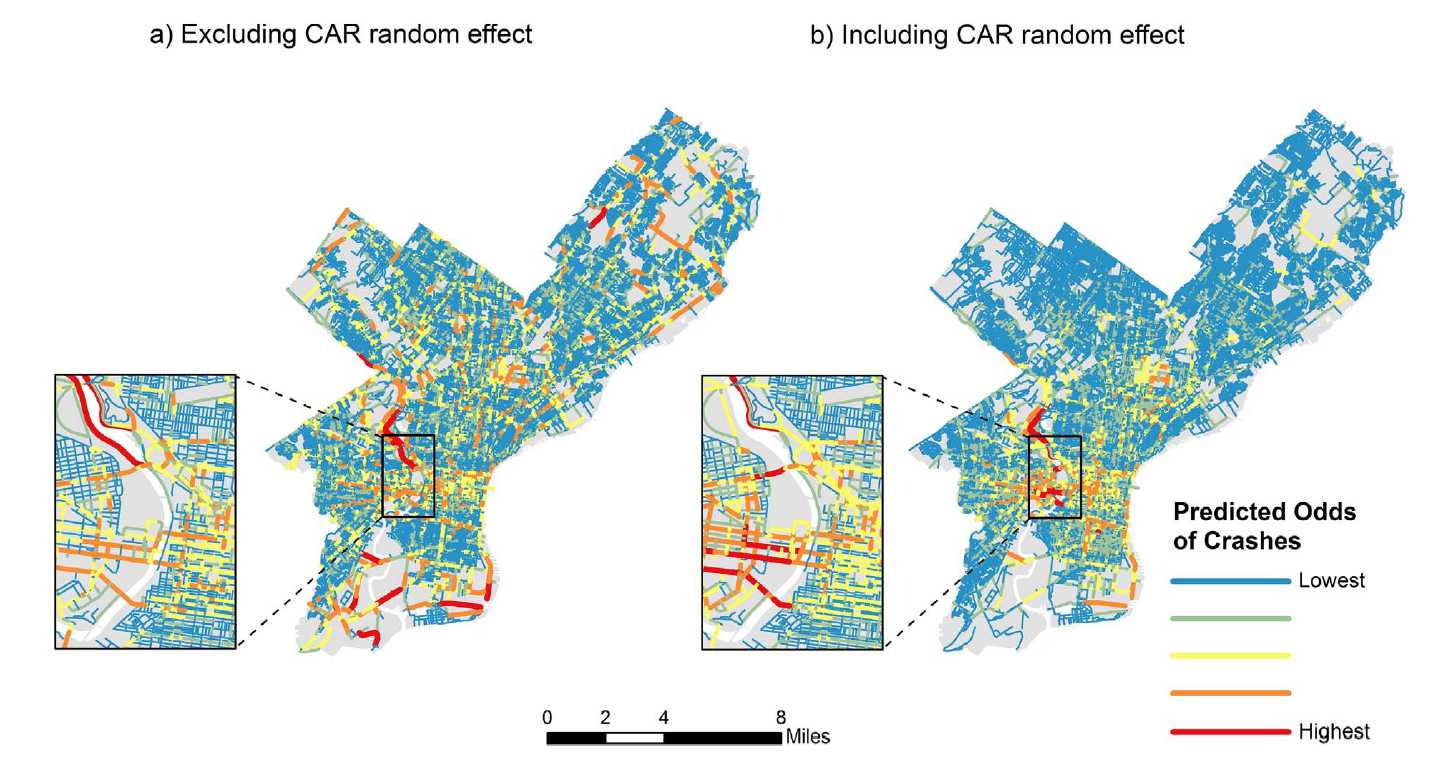
\includegraphics[width=\textwidth]{Plots/Kondor.png}
	\captionsource{(a und b). Berechnete Wahrscheinlichkeiten für Radunfälle in Philadelphia}{
		\cite{Kondo2018}
	}
	\label{kondor}
\end{figure}
Wie viele der bisher genannten Studien konzentrierte sich \cite{Kondo2018} auf eine Stadt, was ein nicht unwesentliches Problem darstellen kann, denn unterscheidet sich der Straßenverkehr von Stadt zu Stadt, wie auch \cite{Goldmann2021} zeigen. Gerade die Ergebnisse aus Philadelphia, einer der fahrradfreundlichsten Städte der USA, lassen sich eventuell nicht eins zu eins auf andere Städte der USA übertragen, da Autofahrer in Philadelphia durch den höheren Verkehr von Fahrrädern an die Rücksichtname gewöhnt sein könnten, die Autofahrer aus Erfahrung walten lassen. Deswegen wäre es ein interessanter Schritt, diese Beobachtungen auf einer Makro Ebene zu tätigen, um zu sehen, welche Faktoren Städte übergreifend für Fahrrad Sicherheit sorgen.\\
Genau dies machen \cite{Saha2018}, in dem Sie eine Analyse Floridas auf Zensus Block Größe vornehmen. Bei dieser Analyse stellen sie eine räumliche Konzentration und keine Gleichverteilung von Unfällen fest. Um dies zu erklären nutzen die Autoren ein bedingtes autoregressives Modell mit bedingten Variablen der Demographie, sozioökonimischen Daten, Straßen Infrastruktur und Radverkehr Charakteristiken. Davon wurden 21 Variablen als einflussreich identifiziert z.B. Bevölkerung, Alterskohorten, Autobesitz von Haushalten, Straßennetz Dichte oder Fahrradtour Intensität. Für das Modell worden Zensus Daten von 2011 bis 2014 verwendet, zu sehen auch in der Abbildung \ref{SAHA}.  
\begin{figure}[!ht]
	\centering
	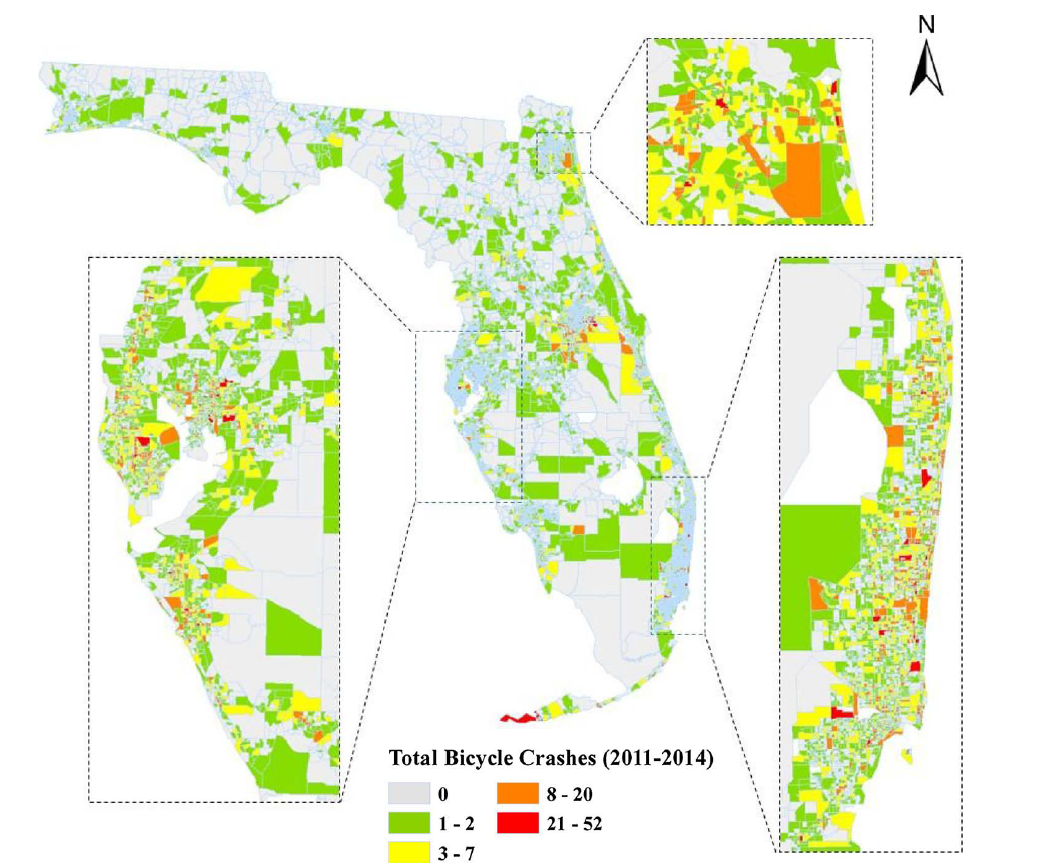
\includegraphics[width=\textwidth]{Plots/saha.png}
	\captionsource{Räumliche Verteilung aller Fahrradunfälle (2011–2014) nach Zensus Blöcken in Florida.}{
		\cite{Saha2018}
	}
	\label{SAHA}
\end{figure}
Gerade die letzten zwei Studien zeigen, wie interessant die räumliche Verteilung von Fahrradunfällen ist und \cite{Kondo2018} zeigen auch das Verkehrsvolumen als Faktor der Unfallwahrscheinlichkeit.\\
Neben all dem ist interessant, dass \cite{Kondo2018} darauf verweisen, dass Unfallsicherheit ein starker Prädikator sei für den Fahrradverkehr laut \cite{Pucher2010}, \cite{Thomas2013} und \cite{Winters2010}. Dies ist eine gute Überleitung auf das nächste Thema. Die bisherige Betrachtung beschäftigte sich mit den Daten, die man verwenden kann für die abhängige Variable des Modells, dass am Ende dieses Projekts entstehen soll. Doch für eine zuverlässige Vorhersage braucht es Prädikatoren. Diese sind in der Literatur zu finden.

\subsection{Sonstige Aspekte}

Eine weitere interessante Datenquelle, die wir z.B. schon bei \cite{Alattar2021} kennen gelernt haben, ist Open Street Map. Dies ist ein 2004 gegründetes gemeinnütziges Projekt, dass das Ziel verfolgt Kartenmaterial zu sammeln und online allen frei zur Verfügung zu stellen. Hier sind Daten über Straßen, Eisenbahnen, Flüsse, Wälder, Häuser und vielem weiteren zu finden. Auch \cite{Carl2015} nutzt die frei verfügbaren Daten zu Höhenmetern des Geländes von Open Street Map, um die Planung von mehrtägigen Fahrradtouren zu erleichtern, die der Erholung dienen. Deswegen ist dieses Paper für die Frage dieser Hausarbeit weniger interessant, die Idee, diese Art von Daten zu verwenden, aber könnte hilfreich sein. Dass aber die Topographie eine Rolle auch für den Pendler Verkehr spielt, zeigt \cite{Rietveld2004}.\\
Vor allem nützlich aber ist diese Datenquelle, wenn man wie \cite{Goldmann2021} mehrere Städte untersuchen möchte und deren Unterschiede. Sie verwenden nicht nur Daten zur Demographie, sondern auch zur Topographie oder auch zur Dichte von Radwegen und Haltestopps des öffentlichen Nahverkehrs.


\chapter{Zusammensetzung des Datensatz}

Das vorherige Kapital zeigte den aktuellen Stand der Forschung zum Aufkommen des Fahrradverkehrs und endete mit einer Einschätzung, an welchen Studien sich diese Masterarbeit orientieren muss, um die gestellte Forschungsfrage zu beantworten. Darauf baute auch die Beschaffung von Daten für das Modell dieser Arbeit auf, angefangen über die Daten der Fahrradzähler, Daten zum Wetter, demographischen Daten und Daten der vorhandenen Infrastruktur erhoben durch Open Street Map. Einen tieferen Einblick über die Datenbeschaffung und die Verteilung von Daten mit zugehörigen Abbildung beinhaltet dieses Kapitel.\\
Die Datenbeschaffung an sich beschränkt sich allein auf Deutschland aus Gründen der Einfachheit. Bestimmte Daten wie Daten zum Wetter und zur Demographie lassen sich so allein von einer Datenquelle beschaffen in diesem Fall dem Deutschen Wetter Dienst und dem statistischen Bumdesamt DESTATIS. Der Nachteil davon ist, dass wiederum alle Aussagen des Modells allein für Deutschland gültig sind, da dieser Rahmen die Evaluierung für andere Regionen der Welt nicht zu lässt.

\section{Fahrradzähler}

Notwendige Grundlage der Forschung sind Daten von Fahrradzählstationen. Dankbarerweise stellen diese Daten viele Kommunen öffentlich zur Verfügung oder teilen diese auf Nachfrage. Insgesamt befinden sich Daten von 13 deutschen Städten im Datensatz, darunter Berlin, Bochum, Bonn, Bremen, Darmstadt, Düsseldorf, Hamburg, Mannheim, München, Münster, Oberhausen, Rostock und Siegen.

\section{Wetterdaten}
\section{Demographische Statistiken}
\section{Open Street Map Daten}
\subsection{Ausgewählte POIs}
\subsection{Ausgestaltung des öffentlichen Verkehrs}
\subsection{Straßentypen}
\subsection{Sonstige}

\chapter{Verwendete Methoden}

Das vorangegangene Kapitel gab einen genauen Überblick über die bestehende Literatur, die sich mit der Vorhersage des Aufkommens von Fahrrädern in urbanen Zentren beschäftigt. Immer häufiger wurden dabei Machine Learning Methoden zur Schätzung eines Modells verwendet. Um die Übersichtlichkeit der Arbeit zu gewährleisten, wurden Erläuterungen, über die verschiedenen verwendeten Methoden, bis zu diesem Zeitpunkt aufgespart, um einen gegliederten Überblick zu ermöglichen.\\
Im Folgendem wird die Funktionsweise von Regressionssystemen, Support Vector Systemen, Entscheidungsbaum Varianten und neuronalen Netzwerken erklärt. Die Auswahl dieser Schwerpunkte beruht auf der Verwendung in der bisher dargestellten Literatur. Hat man ein geeignetes Modell ausgewählt, lässt sich dessen Effizienz mit dem richtigen Validierungsverfahren noch weiter steigern. Deswegen beinhaltet dieses Kapitell ebenfalls eine kurze Erläuterung der Cross Validation.

\section{Problem zur Autokorrelation}

\section{OLS Regression}

Einer der einfachsten und geläufigsten Methoden ist die Regressionsanalyse. So nutzen \cite{Holmgren2017}, \cite{Alattar2021} und \cite{Gao2022} z.B. ein lineares Regressionssystem und \cite{Wessel2020} ein log-lineares sowie ein negativ binomiales Regressionssystem.\\
Das Prinzip einer einfachen OLS (Ordinary Least Square) Regression besteht darin, den Zusammenhang zwischen zwei Variablen zu finden, der die Summe der quadrierten Fehlerterme, also die Abweichung tatsächlicher Beobachtungen zur Regressionsgerade, minimiert. Als Maß zur Validierung eines solchen Modells ließe sich z.B. das Bestimmtheitsmaß R$^2$ nutzen, also der Anteil der Streuung, der durch die Regression erklärt werden kann, aber auch z.B. die Wurzel der summierten quadratischen Fehler (RMSE). Ein solches Fehlermaß oder Bestimmtheitsmaß, dass die Performance des Modells bewertet ist nützlich, einen Vergleich zu ziehen, verwendet man mehrere Modelle, wie es zB \cite{Holmgren2017}, \cite{Broucke2019} oder \cite{Gao2022} machen.

\section{Support Vector Regression}


In der bisher betrachteten Literatur haben \cite{Holmgren2017}, \cite{Broucke2019}, \cite{Xu2013} und \cite{Gao2022} Support Vector Machines bzw Support Vector Regressionen verwendet. \cite{Pisner2020} schildern Support Vector Machines als eine supervised Calssification Methode, die eine Hyperebene nutzt, um Daten nach unterschiedlichen Ausprägungsmustern zu trennen und so den jeweiligen Klassen zu zuordnen. Diese Vorgehensweise ist auch dargestellt in Abbildung \ref{SVM}. Nun könnte diese Trennlinie, auch Hyperplane genannt, so gewählt werden, dass sie das Margin, also den Abstand zwischen der Trennlinie selbst und der nächstgelegenen Beobachtung, maximiert. Dieses Vorgehen wird auch als Maximum Margin Classification bezeichnet. Jedoch falls innerhalb des maximalen Margin-Bereichs eine neue zufällige Beobachtung hinzu kommt, dann führt diese zu einer starken Veränderung der Trennlinie selbst. Ausreißer Daten können so zu einer starken Verzerrung führen und eine Generalisierbarkeit wäre nicht gegeben.
\begin{figure}[!ht]
	\centering
	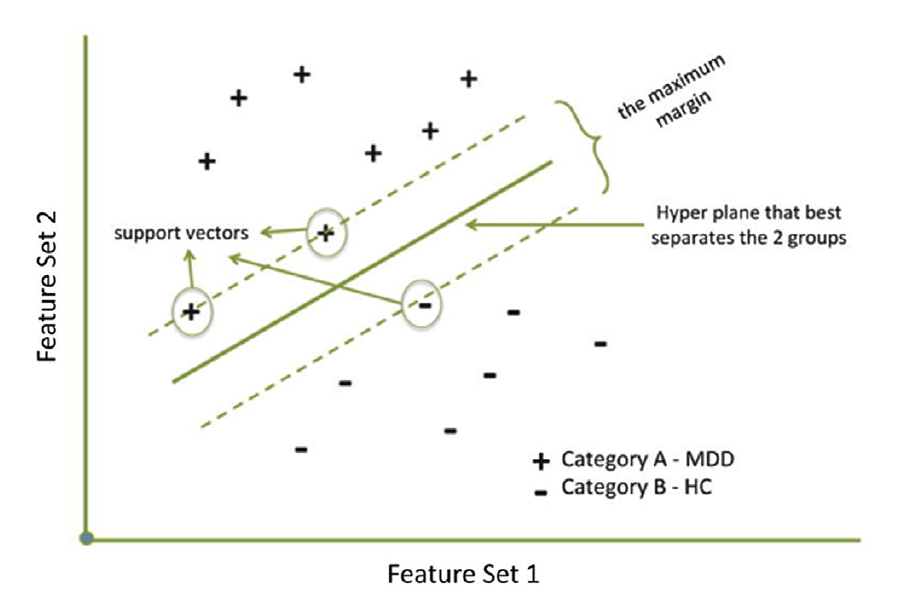
\includegraphics[width=\textwidth]{Plots/SVM.png}
	\captionsource{Hyperebenen (Hyperplanes) in Support Vector Machines}{
		\cite{Pisner2020}
	}
	\label{SVM}
\end{figure}\\
Deswegen nutzt man oft soft Margins, die die Missklassifikation von Ausreißern zu lassen. Dabei stellt $\xi$ die Variable für die Toleranz von Missklassifikationen dar, auch oft Slack Variable genannt. Ist $\xi=0$ so erhalten wir ein hard Margin Classifier.
\begin{figure}[!ht]
	\centering
	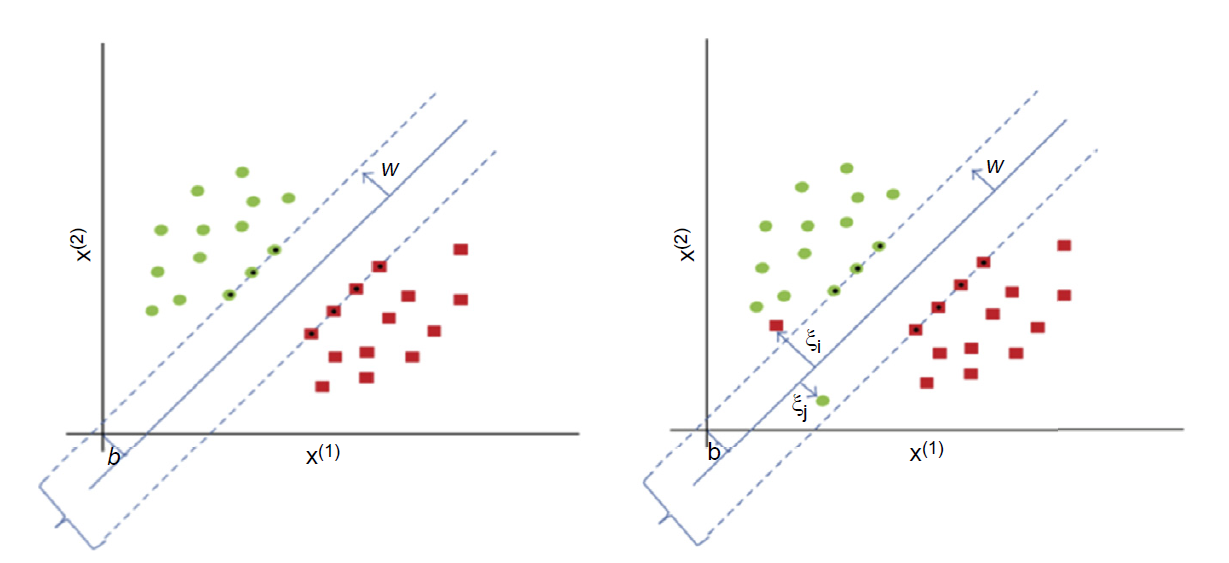
\includegraphics[width=\textwidth]{Plots/SVM2.png}
	\captionsource{Soft Margins in Support Vector Machines}{
		\cite{Pisner2020}
	}
	\label{SVM2}
\end{figure}\\
Mathematisch formulieren \cite{James2013SVM} eine Hyperplane in einem p-dimensionalen Raum wie folgt:
\begin{equation}
	\label{SVM:Hyperplane}
	\beta_0 + \beta_1 X_1 + \beta_2 X_2 + ... + \beta_p X_p = 0
\end{equation}
Dabei liegt der Normalenvektor $\beta=(\beta_1, \beta_2, ..., \beta_p)$ in der orthogonalen Richtung zur Hyperplane. Das Optimierungsproblem hinter der soft Margin ($M$) Klassifikation sieht wie folgt aus:
\begin{equation}
	\label{SVM:SoftMarginClassifier}
	\begin{aligned}
		&\underset{\beta_0, \beta_1, ... , \beta_p,M,\xi_1,...,\xi_n}{\text{max}}M \\
		&\text{udN}\: \sum_{j=0}^p\beta_j^2=1, \\
		&y_i(\beta_0 + \beta_1 x_{i1} + ... + \beta_{ip}) \geq M(1-\xi_i),\\
		&\xi_i \geq 0, \sum_{i=0}^n\xi_i \leq D,
	\end{aligned} 
\end{equation}
Hier taucht nun die Slack Variable auf, die einen Toleranzbereich für Missklassifikation ermöglicht. Setzt man $\xi=0$, erhält man einen hard Margin Classifier. D ist ein nichtlinearer Tuning Parameter. Natürlich kann man in der Funktion des Hyperplanes (\ref{SVM:Hyperplane}) Polynomiale aufnehmen und so einen nicht linearen Classifier erhalten.\\
Grundlegendes Problem ist nun, dass in der Vorhersage des innerstädtischen Fahrradaufkommens kein Klassifikationsproblem besteht, so wie es eine Support Vector Machine lösen würde. Deswegen bietet es sich an, eine Support Vector Regression zu nutzen, so wie es z.B. \cite{Holmgren2017} macht. Während herkömmliche OLS Regression die summierten quadratischen Fehlerterme minimiert, minimiert Support Vector Regression, so beschreiben es \cite{Awad2015}, eine Loss Function, die Fehlvorhersagen bestraft. Dieser Vorgang ist auch eine Verallgemeinerung des bisher beschriebenen Klassifikations Algorithmus.\\ 
\begin{figure}[!ht]
	\centering
	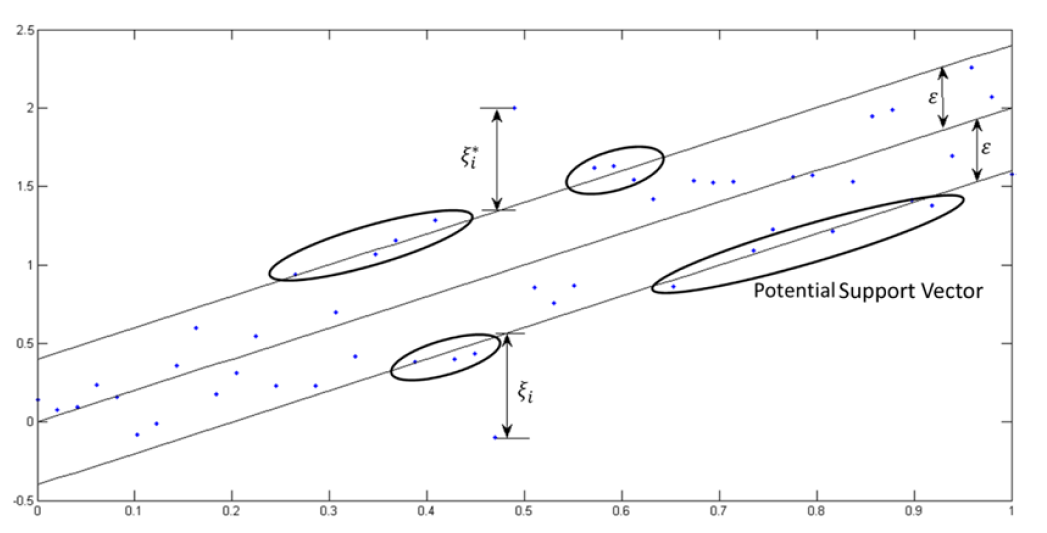
\includegraphics[width=\textwidth]{Plots/SVM3.png}
	\captionsource{Eindimensionale lineare SVR}{
		\cite{Awad2015}
	}
	\label{SVM3}
\end{figure}\\
Wo im Soft Margin Classifier $\xi$ genutzt worden ist, um auch Missklassifikationen zuzulassen, wird nun ein unempfindlicher Bereich von $\varepsilon$ um die Hyperplane herum gelegt, sodass ein Großteil der Beobachtungen im eigentlichen Margin Bereich zu finden sind. Aus der Hyperplane, die eigentlich Beobachtungen trennen soll wird so die regressive $\varepsilon$-Tube, eine wertbeständige Funktion. Dargestellt ist dies auch in der Abbildung \ref{SVM3}.\\
Die Slack Variable $\xi$ wird so zur Toleranz Variable für Ausreißer von der $\varepsilon$-Tube und so zum Bestandteil der Loss Function, die man versucht zu minimieren. Zusammen mit C der Gewichtung der Minimierung ergibt das:
\begin{equation}
	\label{SVM:Regression}
	\begin{aligned}
		&\underset{\beta_0, \beta_1, ... , \beta_p,M,\xi_1,...,\xi_n}{\text{min}}\frac{1}{2}||\beta||^2 + C\sum_{i=1}^N \xi_i + \xi_i^*\\
		&\text{udN}\; y_i - \beta^T x_i \leq \varepsilon + \xi_i^*, \; i=1...N\\
		&\beta^T x_i - y_i \leq \varepsilon + \xi_i^, \; i=1...N\\
		&\xi_i, \xi_i^* \geq 0, \; i=1...N
	\end{aligned} 
\end{equation}
Der Vorteil dieser Vorgehensweise ist, dass man durch den Optimierungsprozess ein Modell erhält, das sehr robust auf Ausreißer reagiert trotzt hoher Präzession durch die Nutzung von $\xi$.

\section{Random Forests Regression}

Entscheidungsbaum Methoden finden sich bei \cite{Holmgren2017}, \cite{Broucke2019}, \cite{Mitchell2018PredictingBT} und \cite{Gao2022}. Dabei sind diese simpel, nicht immer aber besonders präzise so \cite{James2013TBM}. Es sei denn man nutzt komplexere Weiterentwicklungen wie Random Forests. Diese nutzen auch \cite{Holmgren2017}, \cite{Broucke2019} und \cite{Mitchell2018PredictingBT}.\\ 
Ein Vorteil für diese Hausarbeit ist weiter, dass Entscheidungsbaum Methoden sowohl zur Klassifikation, als auch zur Regression genutzt werden können so \cite{James2013TBM}. Die Begrifflichkeit rührt von der Struktur in der Entscheidungsbäume Daten aufbereiten, denn ihre Darstellungsweise erinnert an eine umgedrehte Baumkrone, in der jede Astgabelungen ein Statement darstellt, welches mit wahr oder falsch beantwortet werden kann. Die Beobachtungen aus dem Datensatz folgen entlang ihrer Ausprägung verschiedenen Astgabelungen und werden so einer Vorhersage zugeordnet. Dies kann z.B. aussehen, wie in Abbildung \ref{DTM1}.
\begin{figure}[!ht]
	\centering
	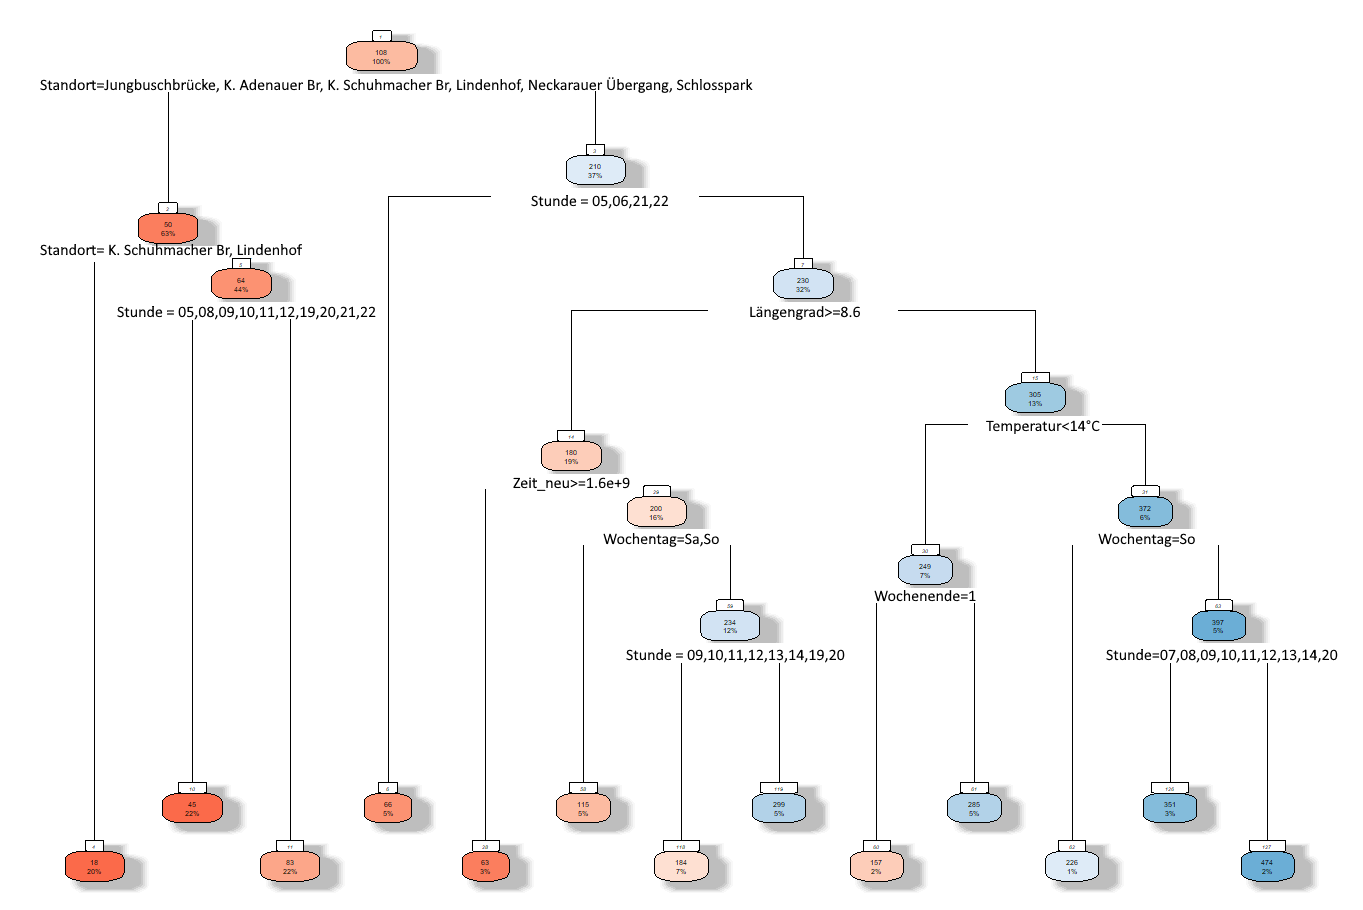
\includegraphics[width=16cm]{Plots/Entscheidungsbaum.png}
	\captionsource{Ein Entscheidungsbaum basierend auf Daten von Fahrradzählstationen in Mannheim und Daten des DWD 2016 bis 2022.}{
		Eigene Darstellung
	}
	\label{DTM1}
\end{figure}\\
Durch diese Entscheidungsgrenzen unterteilt der Entscheidungsbaum den Prädiaktorenraum in distinkte sich nicht überlappende Regionen $R_1,R_2,...,R_J$. Das Optimierungsproblem besteht nun darin, $R_1,R_2,...,R_J$ so zu wählen, dass die Summe der quadrierten Residuen (RSS) minimiert wird: 
\begin{equation}
	\label{TDM:TreeOptimization}
	\sum_{j=1}^J\sum_{i\in R_j}(y_i - \hat{y}_{R_j})^2
\end{equation}
Auf diese Weise lässt sich ein Entscheidungsbaum erstellen. Bei den zuvor angesprochenen Random Forests wird diese Vorgehensweise mit einem Bootstraps Verfahren kombiniert. Bootstraping bedeutet, dass durch zufällige Ziehungen von Beobachtungen aus einem bestehenden Datensatz, wobei mehrfach Ziehungen erlaubt sind, ein neuer Bootstraps Datensatz erstellt wird, der dem ursprünglichen Datensatz ähnelt, jedoch davon abweicht. Diese Praxis führt man mehrere male durch und wendet auf jeden Bootstraps Datensatz einen Entscheidungsbaum an, so das man eine große Anzahl von Entscheidungsbäumen erhält. Möchte man nun auf neuen Beobachtungen eine Vorhersage treffen, lässt man diese durch die Bootstraps Entscheidungsbäume laufen, wobei man sich auf die Vorhersage festlegt, die am meisten von den Bootstraps Entscheidungsbäumen bestimmt wurde. Dieses Verfahren führt zu einer deutlichen Steigerung der Vorhersage Genauigkeit.

\section{Neuronale Netze}


Deep Learning Algorithmen und die dazu gehörigen neuronalen Netzwerke sind mit die fortgeschrittenste Form im Bereich des Machine Learnings. Sie tauchen bei \cite{Broucke2019} und \cite{Mitchell2018PredictingBT} auf.
\subsubsection{Aufbau eines neuronalen Netzes}
Zur Verdeutlichung der Funktionsweise von neuronalen Netzwerken beschränkt sich diese Arbeit aufgrund von Übersichtlichkeit auf Single Layer Perceptrons, diese sind die einfachste Form eines neuronalen Netzes und bestehen nur aus einer Schicht von Neuronen. Eine graphische Darstellung eines solchen Netzwerkes ist in Abbildung \ref{NN1} zu sehen.
\begin{figure}[!ht]
	\centering
	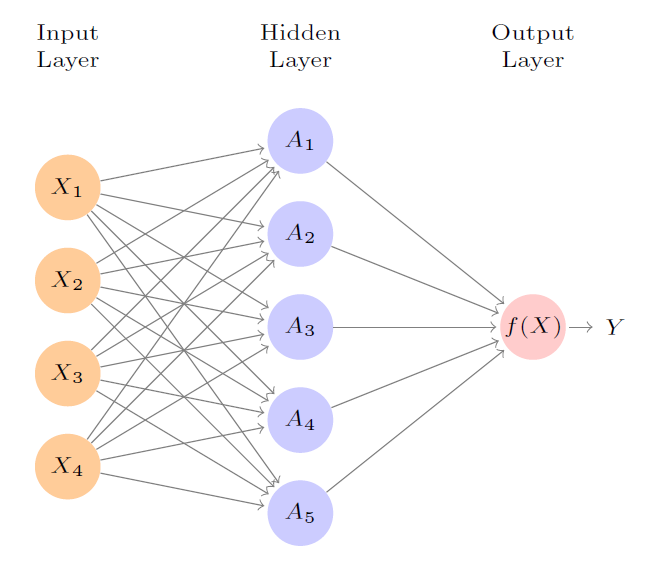
\includegraphics[width=12cm]{Plots/NN1.png}
	\captionsource{Neural network with a single hidden layer}{
		\cite{James2013DL}
	}
	\label{NN1}
\end{figure}\\
Mathematisch ausgedrückt, gleicht dieses Netzwerk einer Vektor Multiplikation. Im Input Vektor (Input Layer), sind die Variablen einer jeden einzelnen Beobachtungen zu finden. Diese werden mit Gewichten im Hidden Layer multipliziert. Wobei jeder einzelner Punkt in diesem Layer, auch Neuron genannt, über ein separates Gewicht verfügt. Diese sind so eingestellt, dass im Output eine möglichst zielgenaue Vorhersage zustande kommt. Als Formel sieht diese Vorgehensweise wie folgt aus:
\begin{equation}
	\label{NN:SingleLayerNetwork}
	\begin{aligned}
		f(x)& = \beta_0 + \sum_{k = 1}^K \beta_k h_k (X)\\
		& = \beta_0  + \sum_{k = 1}^K \beta_k \underbrace{ g(w_{k0} + \sum_{j = 1}^p w_{kj} X_)}_{\text{Aktivierungsfunktion}}
	\end{aligned} 
\end{equation}
Ob und in welchem Umfang die Information, die ein Neuron passiert, weiter gereicht wird, entscheidet die Aktivierungsfunktion $g(z)$. In ihr werden die Informationen des Inputs und die der Gewichte übertragen. Das kann z.B. durch eine Sigmoid Funktion (\ref{NN:Sigmoid}) oder durch eine ReLU (Rectified Linear Unit) Funktion (\ref{NN:ReLU}) geschehen.
\begin{equation}
	\label{NN:Sigmoid}
	g(z)=\frac{e^z}{1+e^z}=\frac{1}{1+e^{-z}}
\end{equation}
\begin{equation}
	\label{NN:ReLU}
	g(z)=\begin{cases}
		0 \; \text{wenn $z<0$}
		\\
		z \; \text{sonst}.
	\end{cases}
\end{equation}
\begin{figure}[!ht]
	\centering
	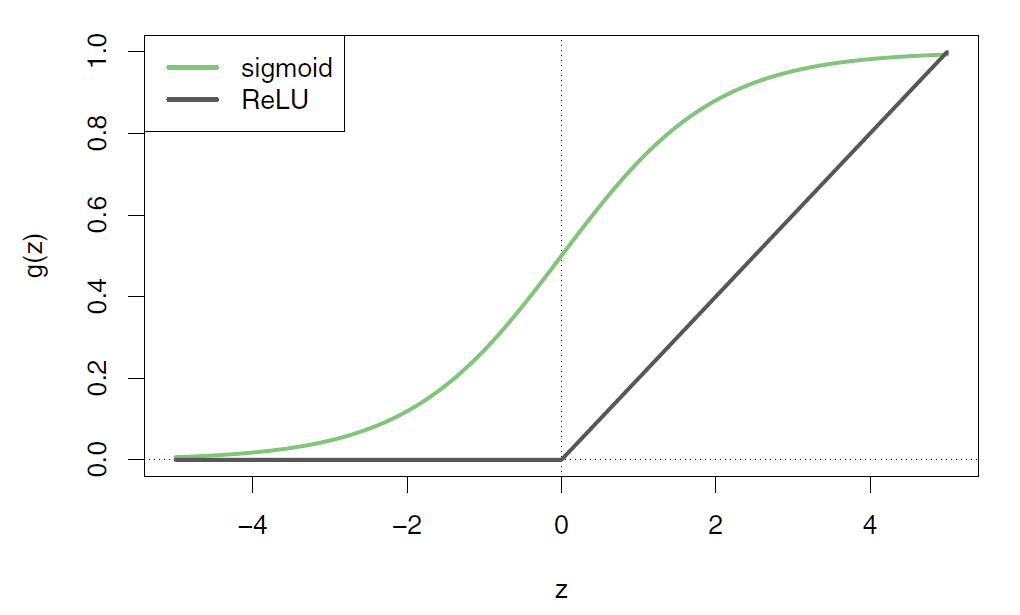
\includegraphics[width=10cm]{Plots/NN2.png}
	\captionsource{Aktivierungsfunktionen}{
		\cite{James2013DL}
	}
	\label{NN2}
\end{figure}\\
Die Sigmoid Funktion wird z.B. auch für die logistische Regression genutzt. Der Vorteil der ReLU Funktion besteht darin, dass Neuronen ausgeschaltet werden, sollte $z$ zu klein sein, wodurch Rechenkraft gespart wird. Zu dem reagiert das Neuronale Netz stärker auf höhere Werte von $z$ und lernt damit schneller.
\subsubsection{Entstehung eines neuronalen Netzes}
Wichtig damit die Aktivierung eines Neurons zur richtigen Vorhersage führt, ist das richtig trainierte Gewicht $w_{kj}$. Sowohl die Parameter $\beta_0, ..., \beta_K$ als auch $w_{10}, ..., w_{Kp}$ müssen trainiert werden. Das Optimierungsproblem dazu besteht in:
\begin{equation}
	\label{NN:Optimization}
	\underset{ \{ w_k \}^K_1 , \beta }{\text{min}}\frac{1}{2}\sum_{i=1}^n (y_i-f(x))^2
\end{equation}
Um diese Optimierung vorzunehmen verwendet man den Vektor $\theta$, der alle zu optimierenden Variablen enthält. Der Fehlerterm ergibt dann:
\begin{equation}
	\label{NN:ErrorTerm}
	R(\theta)=\frac{1}{2}\sum_{i=1}^n (y_i-f_{\theta}(x))^2 \; \; \text{mit} \; \theta=(\{ w_k \}^K_1,\beta)
\end{equation}
Zu Beginn des Optimierungsprozesses wird $\theta^{t=0}$ angenommen, dass heißt der Vektor beginnt ungewichtet. Darauf hin folgen Wiederholungen eines Prozesses, bei dem ein Vektor $\delta$ gefunden werden muss, sodass $\theta^{t+1}=\theta^t + \delta$ zu $R(\theta^{t+1})<R(\theta^t)$. In jedem Durchlauf dieses Prozess wird $t$ erhöht. Eine eindimensionale Veranschaulichungen dieses Prozesses ist in Abbildung \ref{NN3} zu finden.
\begin{figure}[!ht]
	\centering
	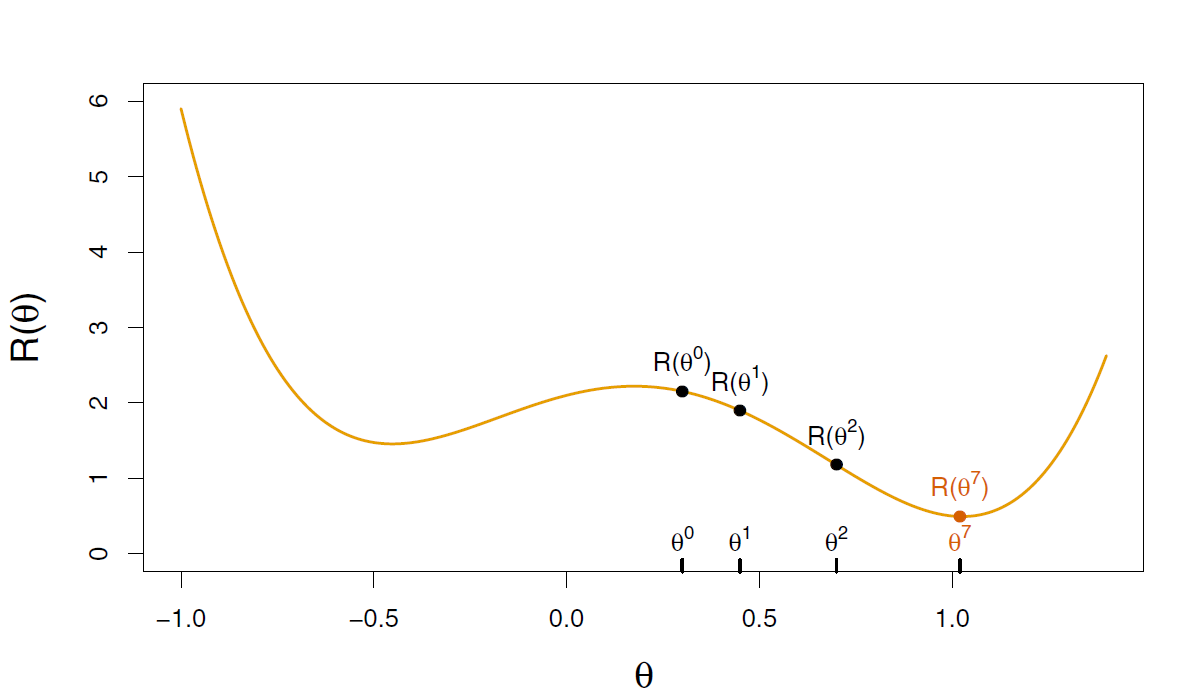
\includegraphics[width=14cm]{Plots/NN3.png}
	\captionsource{Gradiemt Descent}{
		\cite{James2013DL}
	}
	\label{NN3}
\end{figure}\\
Wie kann aber der Vektor $\delta$ gefunden werden, sodass der Fehlerterm gesenkt wird? Dazu muss man den Vektor des Gradienten berechnen:
\begin{equation}
	\label{NN:GradientVector}
	\Delta R(\theta^m)=\frac{\partial R(\theta)}{\partial \theta}|_{\theta=\theta^t}
\end{equation}
Der partielle Vektor der Ableitung der aktuellen Schätzung von $\theta^t$ zeigt aufwärts. Um also $\delta$ zu finden gehen wir in die entgegen gesetzte Richtung gewichtet mit der Lernrate $\rho$. So ergibt sich:
\begin{equation}
	\label{NN:Lernfunktion}
	\theta^{t+m} \leftarrow \theta^m -\rho \Delta R(\theta^m)
\end{equation}
Die Ableitungen des Fehlerterms nach den Gewichten, die wir brauchen, um den Gradientenvektor in \ref{NN:GradientVector} zu bestimmen, kann man durch die Ketten Ableitungsregel vereinfachen:
\begin{equation}
	\label{NN:ChainRule}
	\begin{aligned}
		\frac{\partial R_i(\theta)}{\partial \beta_k}& = \frac{\partial R_i(\theta)}{\partial f_{\theta} (x_i)} \frac{\partial f_{\theta} (x_i)}{\partial \beta_k}\\
		& = -(y_i - f_{\theta})g(z_{ik})\\
		\frac{\partial R_i(\theta)}{\partial w_{kj}}& = \frac{\partial R_i(\theta)}{\partial f_{\theta} (x_i)} \frac{\partial f_{\theta} (x_i)}{\partial g(z_{ik})} \frac{\partial g(z_{ik}) }{\partial z_{ik}} \frac{\partial z_{ik}}{\partial w_{kj}}\\
		& = -(y_i - f_{\theta})\beta_k*g'(z_{ik})x_{ij}\\
		\text{mit}& \; \; z_{ik}=w_{ko}+ \sum^p_{j=1}w_{kj}x_{ij}
	\end{aligned} 
\end{equation}

\section{Feature conditional Validation Set Building}

\section{Cross Validation}

Statistische Modelle wie ein neuronales Netz machen erstaunlich präzise Vorhersagen. Doch wie kann man eine solche Präzession messen? Dafür verantwortlich ist die Validierung. Mittels Maße wie dem Bestimmtheitsmaß R$^2$ oder dem RMSE kann man die Performance der Vorhersagen im Vergleich mit den tatsächlichen Daten messen.\\
Doch wie validiert man die Vorhersagekraft eines Modells auf Daten, mit denen das Modell selbst nicht trainiert worden ist, um zu testen ob das Modell die eigenen Daten nicht overfittet? Hierzu ließe sich der Validation Set Approach nutzen. Teilt man die Beobachtungen in zwei unterschiedlichen Sets zufälligerweise auf, erhält man ein Set, mit dem man ein Modell trainieren kann und eines mit dem man es testen kann.\\
Eine Weiterführung dieses Konzepts ist die Cross Validation. Hier wird der Datensatz nicht in 2 sondern in $k$ viele und gleichgroße Sets unterteilt. Es werden dann $k$ viele Validierungen vorgenommen. Bei jedem Durchlauf wird eines der Sets zur Validierung und die restlichen Sets zum Training verwendet. Das bietet den Vorteil, dass der gesamte Datensatz zur Validierung und zum Training verwendet wird, während beim herkömmlichen Ansatz immer auf ein Teil der Daten verzichtet werden musste.

\chapter{Ergebnisse}


\chapter{Fazit}

Test

\newpage
\addcontentsline{toc}{chapter}{Literaturverzeichnis}
\bibliography{bib1}

\end{document}

